\chapter{Proposing attacks with a model}\label{ch:proposals}

Every assessment in this book rests on a declared list of attacks, and the list is
written by people. People miss things. A natural response is to let a model write
part of the list: a network that learns from past attacks where the risk is high, or
a large language model that has read the literature on re-identification and can
propose scenarios an analyst would not think of. The belief behind that response has
two parts, and in its strongest form both sound right. A model that proposes attacks
makes the audit stronger, because more and better-aimed attacks can only find more
of what is there. And a large language model will find attacks that random search
misses, because it brings knowledge that a random draw does not have.

The repository tested both parts, and neither survived as stated. On 30 state
samples of a public Census file, a neural search that learned from measured attacks
confirmed almost every setting it chose as high risk, 31.57 of 32, and covered fewer
distinct kinds of high-risk scenario than a scrambled Sobol sequence that learned
nothing: 10.07 scenario cells against 13.83.
% source: paper/generated/table_public_search.tex
A small open-weight language model given the same budget covered 6.05 cells against
13.65 for Sobol on the states where it produced a valid answer, because it copied the
front of the list it was shown.
% source: paper/generated/table_public_search_llm.tex
And on the credit register of Chapter~\ref{ch:credit}, a logistic model saved as many
audit draws as the network it was meant to be a baseline for.
% source: paper/generated/table_neural_pipeline.tex

This chapter asks one question: \emph{what can a model that proposes attacks add to a
release decision, and what has to be kept out of its reach for the decision to stay
valid?} The answer is built in four steps. A network can plan an audit and make it
cheaper without touching its error bound. A language model can enter only as an
injector of scenarios into a closed network, through review and measurement. The
experiments that test whether either finds more risk are reported in full, including
the ones that failed. And the provenance ledger and a penetration test show what the
record must carry for an auditor to trust any of it.

\section{Two jobs a model might do}\label{c14:sec-jobs}

A model can enter an audit in two places. It can help \emph{plan} an audit whose
attacks are already declared: predict how each declared attack will fare at each
candidate setting, and so choose where to start and how much to bet on each draw. Or
it can help \emph{search}: propose new scenarios, new adversaries, new settings, and
so change what is declared. Planning changes the cost of the audit. Search changes
its scope. Neither job, done well or badly, is the job of deciding.

The book's decision rule fixes where the decision lies. For a proposed setting
$\theta$ and a finite declared set $\mathcal J$ of scenarios, each fixing an adversary,
a harm, a target group and a vintage, let $r_j(\theta)$ be the probability that one
fresh attack under scenario $j$ succeeds, and let $\overline r_j(\theta)$ be an upper
confidence bound from an audit. The release is admissible when every audited margin
\begin{equation}\label{c14:eq-margin}
z_j(\theta) = 1 - \frac{\overline r_j(\theta)}{\tau_j}, \qquad j \in \mathcal J,
\end{equation}
is nonnegative, where $\tau_j$ is the tolerance for scenario $j$. A coordinate that
was never audited receives $\overline r_j = 1$ and fails. The vector of margins is what
the decision record carries, because its minimum alone hides which group or which
pooled attack constrains the release.
% source: paper/neural_section.tex eq. trust-position
A model's output is a predicted attack frequency. It is not an audited margin, and
nothing a model writes can stand in for $\overline r_j$.

The Bank's data innovation group sends the release committee a proposal: a language
model that drafts attack scenarios for each release, so that Naledi's lists would no
longer depend on what she happens to think of. The chair forwards it to her with one
line: does this make the audit stronger? Naledi answers that she does not know yet,
and that the repository has the experiments that would tell her.

\section{A network that plans the audit}\label{c14:sec-pipeline}

The release chain of Chapter~\ref{ch:monitoring} audits floors from the strictest
down, and at every draw it needs a bet, and it needs a floor at which to start. The
neural release pipeline supplies both from a network fitted to earlier attacks. It
runs in four stages, shown in Figure~\ref{c14:fig-pipeline}, and keeps their evidence
apart.

\begin{figure}[ht]
\centering
\begin{tikzpicture}[font=\small,x=1cm,y=1cm]
  \tikzset{st/.style={draw,rounded corners=2pt,align=center,text width=2.8cm,minimum height=1.5cm}}
  \node[st,fill=gray!15] (a) at (0,0) {1. Development\\attacks on 25\\floors, own seeds};
  \node[st,fill=gray!15] (b) at (4.9,0) {2. Network fitted\\by binomial\\likelihood};
  \node[st,double,double distance=1.2pt] (c) at (9.8,0) {3. Plan frozen:\\bets, start floor,\\SHA-256 digest};
  \node[st,pattern=north east lines,pattern color=gray!45] (d) at (9.8,-2.6) {4. Release chain\\on fresh targets};
  \node[st] (e) at (4.9,-2.6) {Floor certified,\\or none};
  \node[st] (f) at (0,-2.6) {Reserve chain\\from $k_{\min}=300$};
  \draw[->] (a) -- node[above,font=\scriptsize]{counts} (b);
  \draw[->] (b) -- node[below,font=\scriptsize]{predicted} (c);
  \draw[->] (c) -- node[right,font=\scriptsize,align=left]{fixed before\\outcomes} (d);
  \draw[->] (d) -- (e);
  \draw[->,dashed] (d.south) -- (9.8,-3.8) -- node[below,font=\scriptsize]{first floor fails} (0,-3.8) -- (f.south);
  \draw[->,dashed] (f) -- (e);
  \draw[densely dotted,thick] (-1.75,-1.0) rectangle (6.65,1.0);
  \node[anchor=south west,font=\scriptsize] at (-1.75,1.0) {development evidence only};
\end{tikzpicture}
\caption{The neural release pipeline. Shaded boxes use development attacks only; the
double box is the plan, frozen with its digest before any final outcome exists; the
hatched box is the only stage whose outcomes can certify a floor. Dashed arrows are
the reserve path, used only if the chain fails at its first floor.}
\label{c14:fig-pipeline}
\end{figure}

In the first stage the three declared attacks of Chapter~\ref{ch:credit} (one release
with one reading; six vintages with one reading and the history; six vintages with a
reading per vintage and the history) are run on a dense grid of 25 floors with 400
development targets each, on seeds the final audit never uses. In the second, a
network with two hidden layers of 16 units is fitted to these counts by the binomial
likelihood, one output per declared attack, with a third of the floors held out for
early stopping; a logistic model is fitted to the same counts as a baseline. The
features are ones an institution can compute from the register without running an
attack: the floor, the share of loans kept, the mean size of the released cells, and
the share of released loans not live in every vintage.
% source: paper/bis_ifc_full.tex l.2426-2438; src/privacy_risk/neural_pipeline.py (DEVELOPMENT_LEVELS has 25 floors, FEATURES)

In the third stage, before any final outcome exists, the fitted model predicts every
attack's success at every floor of the 13-floor release grid. The plan records these
predictions, a bet for each draw derived from them, the predicted floor (the last
floor, from 300 down, at which every predicted risk lies below the tolerance) and a
start floor one step stricter. The plan is serialised and hashed with SHA-256; the
network's plan in the reported run has the digest beginning \texttt{982f0d60} and the
logistic plan the digest beginning \texttt{ac74ebfb}. In the fourth stage the release
chain audits the plan on fresh targets. If it fails at its first floor, a reserve of a
fifth of the error budget runs a second chain from $k_{\min}=300$.
% source: src/privacy_risk/neural_pipeline.py (LEVELS has 13 floors; plan sha256; reserve 0.2); artifacts-neural/neural_pipeline.json (plans: sha256)

Because every bet is fixed before its outcome and the order of the chain is fixed at
registration, the network's accuracy does not enter the error bound. A poor network
costs attacks. It cannot raise the chance of certifying an unsafe floor. The argument
for the betting chain is the test-martingale argument of
Chapter~\ref{ch:monitoring}; the version for a fixed family of exact bounds, which
SENTRY-R below uses, is Proposition~\ref{c14:prop-gate}.

\begin{proposition}[Selection-safe certification]\label{c14:prop-gate}
Let $\mathcal D$ be all development information: every development attack, every
proposal, every model fitted and every tuning choice. Conditional on $\mathcal D$, let
a finite family of $M$ pairs $(\theta, j)$ of candidate setting and scenario, their
tolerances $\tau_j$ and their trial counts $B_{\theta j}$ be fixed, and suppose each
final count satisfies $K_{\theta j} \mid \mathcal D \sim \mathrm{Binom}(B_{\theta j},
r_j(\theta))$. Let $\overline r_{\theta j}$ be the exact one-sided Clopper--Pearson
upper bound at level $\alpha/M$. Then, with probability at least $1-\alpha$,
$r_j(\theta) \le \overline r_{\theta j}$ for every pair at once, and any rule that
certifies only candidates whose margins \eqref{c14:eq-margin} are all nonnegative
certifies a candidate with $r_j(\theta) > \tau_j$ for some $j$ with probability at
most $\alpha$. This holds however $\mathcal D$ was produced, including by a model or a
language model used adaptively.
\end{proposition}

Table~\ref{c14:tab-pipeline} compares five designs over 20 attack streams on the same
final draws, at a tolerance of 0.12 and $\alpha = 0.05$. Every design chose 150 in
almost every stream and none chose an unsafe floor. The difference is cost. With bets
from the network the chain used a median of 5{,}620 attacks against 6{,}422 with bets
from the running rate; with the network's start floor as well it used 5{,}044, about a
fifth fewer, and never needed the reserve.
% source: paper/generated/table_neural_pipeline.tex; artifacts-neural/neural_pipeline.json (unsafe_choices 0, reserve_used 0)

\begin{table}[ht]
\centering
\caption{The neural release pipeline on the synthetic credit register: 20 attack
streams, tolerance 0.12, $\alpha=0.05$. All designs are release chains over the
three declared attacks on the same final draws, and differ only in where the bets and
the start floor come from. Floors chosen, with the number of streams in brackets, and
the median number of attacks.}
\label{c14:tab-pipeline}
\small
\begin{tabular}{lrr}
\toprule
Source of bets and start & Floor chosen & Attacks \\
\midrule
Running-rate bets, chain from 300 & 100 (1), 150 (19) & 6{,}422 \\
Logistic bets, chain from 300     & 100 (2), 150 (18) & 5{,}572 \\
Network bets, chain from 300      & 100 (2), 150 (18) & 5{,}620 \\
Logistic bets and start floor     & 100 (1), 150 (19) & 5{,}019 \\
Network bets and start floor      & 100 (1), 150 (19) & 5{,}044 \\
\bottomrule
\end{tabular}
% source: paper/generated/table_neural_pipeline.tex
\end{table}

Depth does not explain the saving. The logistic model's plan saved as many attacks as
the network's, 5{,}019 against 5{,}044, and its predictions were closer to the true
risks. Figure~\ref{c14:fig-predictions} shows what the two models learned. In each
panel the solid line is the network's prediction at the floors of the release grid,
fixed before the final audit, and the dotted line is the true risk estimated from
100{,}000 separate targets per floor. The crosses are the development rates, each from
only 400 attacks, which is all the models saw. Both recover the shape of the three
curves: flat and low for a single release, falling steeply with the floor for the two
pooled attacks, and crossing the tolerance near $k_{\min}=100$ for the full pooled
attack, which is where the true floor lies.

\begin{figure}[ht]
\centering
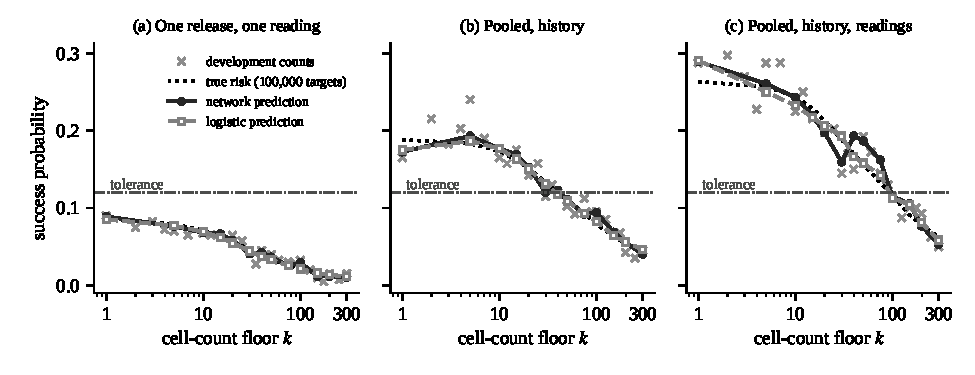
\includegraphics[width=\textwidth]{fig_neural_predictions.pdf}
\caption{Frozen predictions against the truth on the synthetic credit register, for
(a) one release with one reading, (b) six vintages with the history, and (c) six
vintages with the history and a reading per vintage. Crosses are development rates
from 400 attacks each; the dotted line is the true risk from 100{,}000 targets per
floor; filled and open markers are the network's and the logistic model's
predictions; the dash-dotted line is the tolerance.}
\label{c14:fig-predictions}
\end{figure}

Table~\ref{c14:tab-fit} puts numbers on the figure. The two models reach almost the
same held-out log loss, 0.3482 for the network and 0.3480 for the logistic model, and
both predict a floor of 100 and start the chain at 150. Against the true risks over
the 39 coordinates of the release grid, the network's mean error is 0.008 and the
logistic model's 0.004. The network fits the development data as well as the simpler
model and no better, and its largest errors sit in the middle of panel (c), where it
follows the scatter of the development rates. On this register its extra capacity goes
into following noise.
% source: paper/generated/table_neural_fit.tex; paper/bis_ifc_full.tex l.2468-2478

\begin{table}[ht]
\centering
\caption{What the two planning models learned from the development attacks. Log loss
is per development attack; the epoch is where held-out loss was lowest. Errors compare
each frozen prediction with the true risk from 100{,}000 targets over the 39
coordinates of the release grid.}
\label{c14:tab-fit}
\small\setlength{\tabcolsep}{4pt}
\begin{tabular}{lrrrrrrr}
\toprule
 & \multicolumn{2}{c}{Log loss} & & \multicolumn{2}{c}{Error} & \multicolumn{2}{c}{Floor}\\
\cmidrule(lr){2-3}\cmidrule(lr){5-6}\cmidrule(lr){7-8}
Model & Training & Held out & Epoch & Mean & Largest & Predicted & Start \\
\midrule
Network, two hidden layers & 0.3240 & 0.3482 & 1146 & 0.008 & 0.031 & 100 & 150 \\
Logistic model             & 0.3245 & 0.3480 & 2067 & 0.004 & 0.027 & 100 & 150 \\
\bottomrule
\end{tabular}
% source: paper/generated/table_neural_fit.tex
\end{table}

The pipeline keeps the network as its default because its architecture extends to many
more features and declared attacks than this register has, and reports the logistic
model beside it so that a reader can see when depth has not paid. The gain on this
register comes from basing bets and the start floor on development evidence. Any
model that turns development counts into reasonable predictions would have given it.

Grace's question about the pipeline is the one an auditor should ask: how does she
know the plan was fixed before the final draws? The record gives her the plan's
digest and the time it was written, and the final audit refuses to run against a plan
whose digest has changed. Whether that is enough depends on who holds the record, a
point the chapter returns to.

\section{A language model as an injector}\label{c14:sec-sentry}

Planning leaves the declared attacks alone. Search does not, and a language model is
the obvious candidate for search, because it can describe a new adversary, a pooled
release or a new auxiliary source in words. SENTRY-R, short for scenario-enriched
neural triage for release review, is the repository's workflow for letting it do so
without giving it any power over the decision. The phrase the repository uses is
exact: the language model is an injector to a closed neural network.
% source: docs/SENTRY_R.md; README.md
\emph{Closed} names a restricted data path. It does not mean an air gap, frozen
weights or a proof of privacy.
% source: paper/injector_study/main.tex (Introduction)

\begin{figure}[ht]
\centering
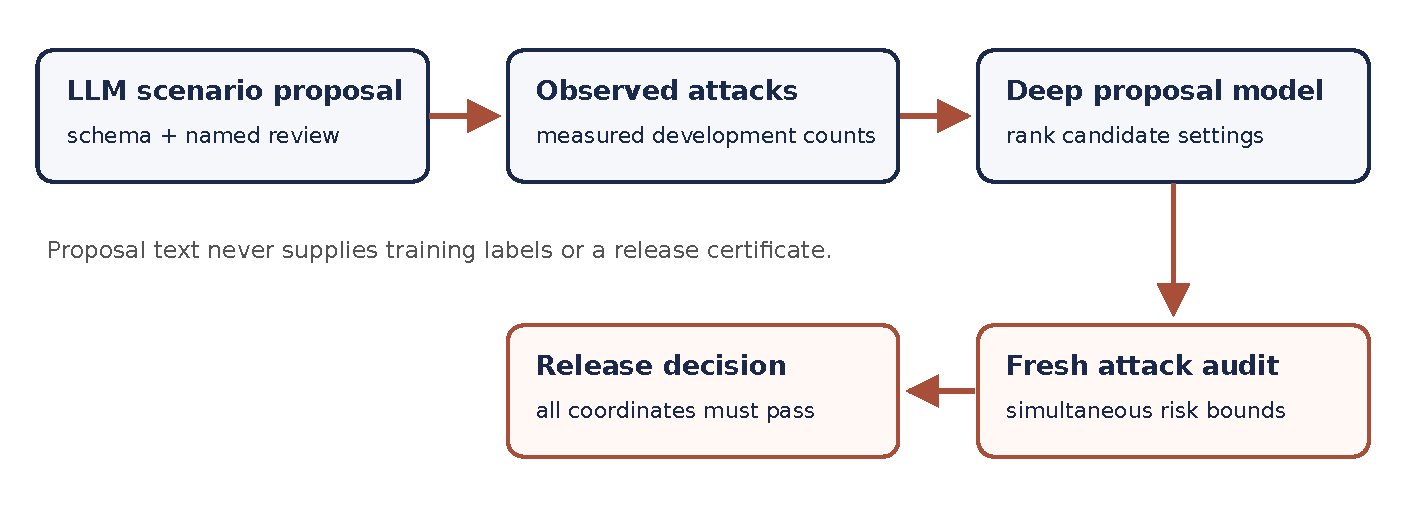
\includegraphics[width=0.95\textwidth]{sentry_r_loop.pdf}
\caption{The SENTRY-R boundary. A scenario proposed by a language model passes a fixed
schema and a named review, and can add a scenario but never an outcome. Only counted
development attacks train the proposal model, whose ranking fixes a shortlist. Only
the fresh final audit, with simultaneous bounds over every coordinate, reaches the
release decision. The upper row is development; the lower row, drawn with a different
fill and border, is the final audit.}
\label{c14:fig-sentry}
\end{figure}

Figure~\ref{c14:fig-sentry} shows the path, and the sequence is strict. The model
returns a JSON array of objects with exactly three fields: an identifier, a scenario
description and a vector of numeric features. A deterministic validator checks the
feature names and their predeclared bounds. The calling code, not the model, writes
the provenance: the model's name as the caller states it and the SHA-256 hash of the
exact prompt sent. A named human reviewer approves or rejects each proposal with a
reason. A separate attack evaluator runs each approved scenario and records the count
of successes and the number of trials. Only those measured counts enter the training
data of the proposal network, which ranks candidate settings and fixes a shortlist.
Only the final audit, on draws no earlier stage has seen, decides. The software refuses
success counts written by the model, refuses responses larger than 256{,}000 bytes
before parsing them, and refuses more than 32 proposals in one batch. The proposal
text is stored as data and never executed.
% source: docs/SENTRY_R.md (intake contract, 256,000-byte cap, 32-proposal cap); src/privacy_risk/sentry_r.py (stage_llm, propose_from_llm)

The reason for refusing a model's counts is statistical, and
Proposition~\ref{c14:prop-labels} states it. A proposal network trained on measured
counts learns the attack's success frequency; trained on anything else, it learns that
thing.

\begin{example}[Three proposals at the intake]\label{c14:ex-intake}
Naledi tried the intake with three answers. The inputs are illustrative; the checks are
the validator's own. A schema declares four features with bounds: geography width from 1
to 100, education width from 1 to 8, minimum cell from 1 to 10, and reading standard
deviation from 0.1 to 2. The model is asked which neighbours could link records, and
returns three answers on three calls. The first proposes a neighbour who knows the area,
the schooling and the income roughly, with features $(1, 4, 1, 0.25)$, and adds a field
\texttt{successes} set to 0. The intake refuses it, because each object must hold exactly
an identifier, a description and the features, and a count is not one of them. The
second drops the count but sets the reading standard deviation to 0.05, below the
declared floor of 0.1; the validator refuses it as out of range. The third is the first
without the count. It is staged with the status ``unverified LLM proposal'', the model
name the caller supplied and the SHA-256 hash of the prompt. It has not yet been
reviewed, and no attack has been run on it.
\end{example}


\begin{proposition}[Only measured counts teach the risk]\label{c14:prop-labels}
For a feature vector $x$ and a trial count $B$ fixed before outcomes, let the training
label be a count $K$ out of $B$ with $\E[K \mid x, B] = B\pi(x)$, and let the
per-pair loss of predicting $p \in (0,1)$ be
$\ell(p) = -[K\log p + (B-K)\log(1-p)]/B_\bullet$ for a normalising constant
$B_\bullet > 0$. Then
\begin{equation}\label{c14:eq-kl}
\E[\ell(p) \mid x,B] - \E[\ell(\pi(x)) \mid x,B]
= \frac{B}{B_\bullet}\,
\mathrm{KL}\bigl(\mathrm{Bern}(\pi(x)) \,\|\, \mathrm{Bern}(p)\bigr) \ \ge 0,
\end{equation}
with equality only at $p = \pi(x)$. If $K$ is replaced by a generated count
$\widetilde K$ with $\E[\widetilde K \mid x,B] = B\widetilde\pi(x)$, the minimiser
becomes $\widetilde\pi(x)$, whatever the attack's true success probability.
\end{proposition}


\begin{example}[A generated label pulls the model away]\label{c14:ex-label}
The inputs are illustrative. At some setting a declared attack succeeds with probability
$\pi = 0.2$. A model trained on measured counts has an expected loss per trial of 0.500
at the prediction 0.2. Suppose a language model's output had been accepted as labels,
with counts that imply $\widetilde\pi = 0.05$. A model that learns those labels predicts
0.05, and against the true attack its expected loss per trial is 0.640. The gap, 0.140,
is the Kullback--Leibler divergence of \eqref{c14:eq-kl} with $B = B_\bullet$, and the
model now reports a quarter of the true risk. Nothing in its fit to the generated labels
warns of this, because it fits them well.
\end{example}

A prompt that asserts a small risk is therefore no evidence of a small risk, however
plausible its prose. The same identity explains the order of the stages: the network
can only be as right about risk as the measured attacks it is trained on, and the
final audit, which the network never sees, is what checks it.

Naledi walked the innovation group through this path with their draft tool open. It let
the model return a success count with each scenario, and the group had expected those
counts to save attack runs. Under the rules above the validator refuses them, and the
group agreed to remove the field before the tool went any further.

\subsection{The provenance ledger}

The workflow is only as good as the record that it was followed. The repository's
provenance ledger appends every stage to one hash-chained file:
budget, proposal, review, measurement, training, freeze, audit. Each entry carries the
hash of the one before and, with a key held by the operator, an HMAC-SHA256 signature
of its own hash. Entries hold digests and identifiers only, never a proposal's text
and never a count. The ledger enforces three rules. Order: a review is refused unless
its proposal is on the chain, a measurement unless an approving review is, a training
run unless every measured proposal it uses is, a freeze unless its model is, and an
audit unless its freeze is. Budget: a programme's error budget is declared once, and
every audit debits its $\alpha$, so a new shortlist after a failed audit costs budget
and does not restart at the nominal level. Closure: once a freeze has been audited, a
training run may not mix its development evidence with evidence measured after the
audit, so an audit outcome cannot steer the next model.
% source: docs/SENTRY_R.md (The provenance ledger)

The budget rule answers a measured danger. In a synthetic experiment with a true risk
of 0.201, a tolerance of 0.2 and 500 trials per attempt, so that every certificate is
false, an operator who retries a failed audit 20 times at the nominal 5 per cent level
certifies in 50.975 per cent of 20{,}000 simulated programmes, with an exact interval of
50.280 to 51.670 per cent. Preallocating a total of 0.05 across the 20 attempts gives
3.875 per cent (3.612 to 4.152).
% source: RESEARCH_BRIEF.md; artifacts-injector/results.json (audit_restarts)
Chapter~\ref{ch:monitoring} treats retries in general; the point here is that a
language model in the development loop is one more source of reasons to try again.

What the ledger cannot do is stated in the repository as plainly as what it can. An
operator who holds the key and can rewrite the file can rewrite the chain. The budget
debit is recorded after outcomes are supplied, so it does not stop a caller from
drawing outcomes outside the ledger and discarding them. Provenance is optional, base
evidence is supplied by the caller, and reviewer and evaluator identities are labels
the caller writes. A deployment needs a registry service with its own storage, keys
and time source, a reservation of budget before any draw, and chain heads anchored
outside the operator's control. That service is specified and not built.
% source: docs/SENTRY_R.md; paper/sentry_r_section.tex; docs/DEPLOYMENT_AND_PENTEST_2026_10_23.md (registry service not built)
The separation applies the principle of separation of privilege: no single party
should hold every key \citep{saltzer1975}.

Four integrity probes, written against the supplied prototype, all failed before
repair: altered measured counts were accepted; altered measured features were
accepted; an injected copy of a validation row could pass once its identifiers were
changed; and file-intake metadata could bypass the response-size limit. The repairs
commit the digest of the full measured row to the keyed chain and check it when a
training artifact is recorded, refuse an injected training vector identical to a
validation vector, and bound file input before parsing. The copy rule can reject
legitimate collisions and does not detect near copies or semantic contamination.
% source: paper/injector_study/main.tex (Evidence-integrity regression experiment); RESEARCH_BRIEF.md; VALIDATION.md

Naledi reads the ledger section twice and writes a note for the chair. The tool the
innovation group proposes can be fitted into the Bank's process, but only behind a
review, an evaluator and a record that the release team does not control. Without
those, a language model in the loop is one more way to retry an audit until it passes.

\section{Does a model find more?}\label{c14:sec-experiments}

Keeping a model away from the decision makes it safe. Whether it makes the audit
stronger is an empirical question, and the repository ran four experiments on it. The
first two are synthetic pilots with no language model at all; they test whether
adding measured scenarios to the training data helps the network. The third tests
whether depth helps the proposal model. The fourth is the public-file search, where a
real language model finally entered.

\subsection{The probability-law pilot}

The first pilot drew labels from a hand-written probability law. Ten paired seeds, two
laws (one additive, one with an interaction), a logistic model and a network with two
hidden layers, 120 base development rows, 80 early-stopping rows and 32 extra measured
rows per augmentation arm, each row with 100 simulated trials, gave 120 model fits.
Three arms were compared: no augmentation, random augmentation, and a hand-written
stress heuristic that deliberately targets a risk corner present in the interaction
law.
% source: RESEARCH_BRIEF.md (Executed experiment); artifacts-injector/results.json (config)

On the shifted test set of the interaction law, augmentation helped. The deep model's
log loss fell from 0.8856 to 0.6252 with random augmentation and to 0.6597 with the
heuristic, paired changes of $-0.2604$ (95 per cent interval $-0.4582$ to $-0.0625$) and
$-0.2259$ ($-0.3889$ to $-0.0629$). The logistic model with heuristic augmentation had
the lowest mean of all, 0.5872.
% source: RESEARCH_BRIEF.md; artifacts-injector/results.json (summaries, law interaction, shift shifted)
The result looks favourable, and the repository warns against reading it that way. The
heuristic's advantage is informed by construction, since it knows where the law puts
the risk, and the intervals are exploratory $t$ intervals over ten seeds with no
adjustment for multiplicity.

\subsection{The executable linkage pilot}

The second pilot replaced the probability law with attacks that were actually run.
Each trial built a synthetic population of 64 people with three quantised
quasi-identifiers, chose a target, produced a noisy auxiliary observation and noisy
released keys from one to four releases, and counted whether nearest-neighbour linkage
named the target. Five paired seeds, 250 shifted test configurations with 1{,}000
trials each, and separate streams for base, stopping, test and augmentation gave
1{,}382{,}000 linkage trials and 30 more model fits.
% source: RESEARCH_BRIEF.md (Executed synthetic record-linkage experiment); VALIDATION.md

The result is negative. Table~\ref{c14:tab-linkage} gives the test log losses.
Augmentation did not establish an improvement over the base for the deep model: the
random-minus-base change was $-0.0133$ with an interval from $-0.0342$ to $+0.0075$, and
the heuristic-minus-base change $-0.0127$ ($-0.0331$ to $+0.0077$). The heuristic made
the logistic model worse, by $+0.0145$ ($+0.0081$ to $+0.0209$).
% source: artifacts-linkage-injector/results.json (summary); RESEARCH_BRIEF.md
This is the pilot the preface refers to, in which augmenting the training data did not
improve the model. Once the labels came from executed attacks in place of a law
written to reward the heuristic, the advantage went away.

\begin{table}[ht]
\centering
\caption{Executable linkage pilot: shifted-test log loss by model and augmentation arm,
mean over five seeds; 1{,}382{,}000 linkage trials. Lower is better.}
\label{c14:tab-linkage}
\small
\begin{tabular}{lrrr}
\toprule
Model & No augmentation & Random augmentation & Heuristic augmentation \\
\midrule
Logistic          & 0.2849 & 0.2908 & 0.2994 \\
Two hidden layers & 0.3038 & 0.2905 & 0.2911 \\
\bottomrule
\end{tabular}
% source: artifacts-linkage-injector/results.json (summary); RESEARCH_BRIEF.md
\end{table}

\subsection{Depth in the proposal model}

The third experiment asked whether depth helps SENTRY-R's proposal model on a toy law
where nothing else is in question. For each of ten seeds it drew three disjoint
programmes: 320 training rows, 100 rows for early stopping and 2{,}000 test rows. Both
models trained until 150 epochs passed without improvement. The logistic model reached
a test log loss of 0.2556 (standard deviation 0.0043 across replicates) and the
three-layer network 0.2576 (0.0047). The paired deep-minus-logistic difference was
0.0020 (0.0014), and the deep model was lower in none of the ten replicates.
% source: paper/generated/table_sentry_benchmark.tex
The table shows that the pipeline runs. It does not show that depth helps, and the
test programmes come from the same law as the training data, so they do not test
shift.

A comparison on public Census records with whole states held out, in which one- and
three-layer networks reached lower test loss than a plain logistic model and a
quadratic logistic model did better still, is in the repository too. Its linear
baselines were not trained to convergence and its differences lie within bootstrap
intervals, so the long-form paper treats it as evidence neither for nor against the
procedure, and so does this book.
% source: paper/generated/table_real_neural.tex; paper/neural_appendix.tex (Exploratory real-data runs)

Naledi sends the chair the linkage table with a two-line summary. The pilots show that
a network can be trained on measured attacks and that the plumbing works. They do not
show that adding proposed scenarios makes the network better at finding risk, and
none of them involved a language model.

\subsection{Searching a public file}\label{c14:sec-public}

The fourth experiment measures search directly, on real records. The source is the
29{,}501-row public \texttt{census2000} extract distributed with the Python
\texttt{wooldridge} package, version 0.5.0. The first 30 encoded state groups with at
least 100 rows were selected before any attack outcome was seen. Within each state the
attacker uses a matching-key prior and an independently perturbed reading of log
income to identify a record drawn uniformly from the released file.
% source: paper/public_search_section.tex; paper/injector_study/main.tex
A setting is a tuple of four declared choices: geographic coarsening (PUMA width 1, 10
or 100), education coarsening (width 1, 2, 4 or 8), the minimum released cell (1, 3, 5
or 10) and the standard deviation of the auxiliary reading (0.1, 0.25, 0.5, 1 or 2),
240 settings in all before excluding those that release fewer than 30 records.
% source: paper/injector_study/main.tex (Methods)

Each state shares 16 warm-start settings and eight early-stopping settings measured
with 64 trials each. Each of four search arms then chooses 32 further settings,
measured with 64 trials each, and every chosen setting receives 300 fresh confirmation
trials. The arms are random search; a domain heuristic that ranks settings by
reciprocal key frequency plus $0.2/(0.1+\text{sd})$; a scrambled Sobol sequence mapped
onto the catalogue; and neural search, which fits a two-hidden-layer network of width
16 to the counts and acquires batches of eight by predicted risk plus 0.15 times the
distance to the nearest measured setting. The total is
$30\{24(64) + 4(32)(64+300)\} = 1{,}443{,}840$ attack trials, with 120 neural fits.
Evaluator cost is matched across arms; total compute is not, since only the neural arm
fits a model.
% source: paper/injector_study/main.tex (Search budget); docs/PAPER_RESULTS_2026_10_23.md

A chosen setting is confirmed high risk only if the exact one-sided lower limit from
its 300 fresh trials exceeds 0.2, at a per-test level of $0.05/128$ for the 32
settings of each of four arms within a state. Conditional on the full search history,
the probability of any false high-risk confirmation within a state is then at most
0.05; the argument is Proposition~\ref{c14:prop-gate} with the direction of the bound
reversed. This is a lower-bound confirmation of excessive risk, not a certificate of
safety, and it controls error within each state, not across all 30.
% source: paper/public_search_section.tex

The primary endpoint is coverage: the number of distinct cells, out of a fixed
taxonomy of 24, that contain at least one confirmed high-risk setting. The cells cross
the three geography levels, education width above or below two, a minimum cell equal
to one or larger, and a reading standard deviation above or below 0.5. The secondary
endpoint is yield: how many of the 32 chosen settings were confirmed.
% source: paper/public_search_section.tex
Table~\ref{c14:tab-public} gives both.

\begin{table}[ht]
\centering
\caption{Public-file search over 30 Census state samples: mean confirmed high-risk
cells (of 24) and confirmed settings (of 32) per state, with the paired-state bootstrap
difference in cells from Sobol and its 95 per cent interval. Neural fits capped at 600
epochs.}
\label{c14:tab-public}
\small
\begin{tabular}{lrrr}
\toprule
Search & Cells & Settings & Difference from Sobol \\
\midrule
Random           & 13.20 & 22.50 & $-0.63$ [$-1.23$, $-0.03$] \\
Domain heuristic & 11.97 & 32.00 & $-1.87$ [$-2.37$, $-1.33$] \\
Scrambled Sobol  & 13.83 & 22.03 & -- \\
Neural search    & 10.07 & 31.57 & $-3.77$ [$-4.43$, $-3.07$] \\
\bottomrule
\end{tabular}
% source: paper/generated/table_public_search.tex
\end{table}

The table splits the arms into two pairs. Sobol and random search fill the space and
cover the most cells, 13.83 and 13.20, while confirming about two thirds of their
settings. The heuristic and neural search aim at risk: the heuristic confirms all 32
settings on average and neural search 31.57, and they cover fewer cells, 11.97 and
10.07. Neural search covers 3.77 fewer cells than Sobol, with a paired interval of
$-4.43$ to $-3.07$. Four of the 120 neural fits had their best epoch at the 600-epoch
cap; a rerun with a cap of 2{,}000 epochs kept the neural mean at 10.07 cells and the
difference at $-3.77$ ($-4.40$ to $-3.07$). It reused the same data and non-neural
draws, so it is a sensitivity check and not a replication.
% source: paper/generated/table_public_search.tex; paper/public_search_section.tex; docs/PAPER_RESULTS_2026_10_23.md

A model that learns where the risk is will keep choosing settings near the risk it has
already found, and so confirm many settings in few places. That is the trade-off between
yield and coverage, and it is the first half of the misconception. A model that
proposes attacks makes the audit more efficient at confirming what it already
suspects; it does not by that fact make the audit find more kinds of failure. The
coverage score favours space filling by construction, and the cells are bins of
declared choices, not attack families, so the result does not show neural search to be
worse for every purpose. It shows that ``finds more high-risk settings'' and ``finds
more of the high-risk space'' are different claims.

\subsection{A language model as the fifth arm}\label{c14:sec-llm}

The first attempt to add a language model failed before it started. A pilot with a
small hosted model saved its prompts in advance and sent its first request, which
returned an HTTP 429 error with no proposals; the account showed no remaining credit,
and collection stopped with no automatic retry. The record keeps the plan, the prompt
hashes and the failed attempt, and states that no result exists from it.
% source: docs/LLM_PILOT_STATUS_2026_10_23.md

The second attempt ran an open-weight model on the author's own machine:
\texttt{qwen3:4b}, a 4.0-billion-parameter model quantised to Q4\_K\_M, served by
Ollama 0.40.9, so that no account, key or charge was involved and nothing left the
machine. The saved per-state prompt was sent byte for byte, with the model's
thinking mode off, temperature 0.3, and decoding constrained to the JSON shape the
prompt asks for. Each state was allowed three attempts with distinct seeds. Generation
took about 36 seconds per state.
% source: docs/LLM_PILOT_LOCAL_2026_10_23.md; paper/generated/numbers_llm_local.json
The constraint fixed the shape of the output and nothing else; every list was still
checked for its count, the distinctness of its tuples and membership of the catalogue.

The model returned a valid list of 32 tuples for 20 of the 30 states, seven of them at
the first attempt. Of 70 attempts, 50 were rejected: 43 for repeated or off-catalogue
tuples and seven for repeated identifiers.
% source: paper/generated/numbers_llm_local.json
All five arms were then rerun on exactly those 20 states, 1{,}195{,}520 attack trials,
with the per-test level at $0.05/160$. Figure~\ref{c14:fig-llm} plots each arm's
coverage against its yield.

\begin{figure}[ht]
\centering
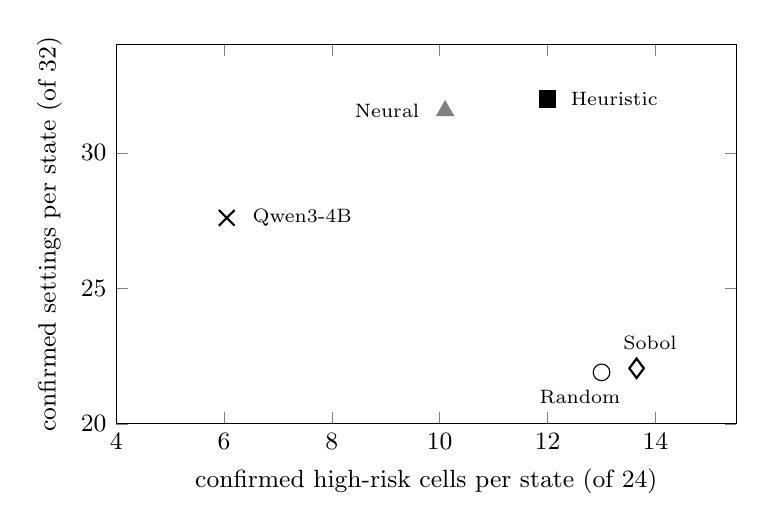
\begin{tikzpicture}
\begin{axis}[width=0.78\textwidth,height=6.4cm,
  xmin=4,xmax=15.5,ymin=20,ymax=34,
  xlabel={confirmed high-risk cells per state (of 24)},
  ylabel={confirmed settings per state (of 32)},
  tick label style={font=\small},label style={font=\small}]
\addplot[only marks,mark=o,mark size=3pt,black] coordinates {(13.00,21.90)};
\addplot[only marks,mark=square*,mark size=3pt,black] coordinates {(12.00,32.00)};
\addplot[only marks,mark=diamond,mark size=3.5pt,black,thick] coordinates {(13.65,22.05)};
\addplot[only marks,mark=triangle*,mark size=3.5pt,gray] coordinates {(10.10,31.55)};
\addplot[only marks,mark=x,mark size=4pt,black,thick] coordinates {(6.05,27.60)};
\node[font=\scriptsize,anchor=north] at (axis cs:12.6,21.6) {Random};
\node[font=\scriptsize,anchor=south] at (axis cs:13.9,22.4) {Sobol};
\node[font=\scriptsize,anchor=west] at (axis cs:12.25,32.0) {Heuristic};
\node[font=\scriptsize,anchor=east] at (axis cs:9.8,31.55) {Neural};
\node[font=\scriptsize,anchor=west] at (axis cs:6.35,27.6) {Qwen3-4B};
\end{axis}
\end{tikzpicture}
% source: paper/generated/table_public_search_llm.tex
\caption{Coverage against yield for five search arms on the 20 Census states for which
the language model returned a valid list (1{,}195{,}520 attack trials). Each arm has its
own marker shape and label. Space-filling arms sit to the right, yield-maximising arms
at the top; the language model sits in neither place.}
\label{c14:fig-llm}
\end{figure}

The baseline ordering of the 30-state run holds on this subset: Sobol 13.65 cells,
random 13.00, heuristic 12.00, neural 10.10. The language model confirmed 27.60 of its
32 settings per state, between the two yield-maximising arms and the two space-filling
ones, but covered only 6.05 cells, 7.60 fewer than Sobol with a paired interval of
$-8.30$ to $-6.80$.
% source: paper/generated/table_public_search_llm.tex
The proposals show why. In 19 of the 20 states every tuple the model chose sat at the
finest geography, and the lists followed the catalogue's own order. The model read the
catalogue as a list to copy and not as a space to search. Its tuples were high risk,
because the finest geography is where the risk is, and they occupied a quarter of the
cells.
% source: docs/LLM_PILOT_LOCAL_2026_10_23.md; paper/generated/numbers_llm_local.json (states_all_finest_geography 19)

This is the second half of the misconception, and the experiment settles less of it
than the first. It settles that a four-billion-parameter open-weight model, under this
fixed prompt, adds no coverage over quasi-random or neural search here and often fails
to produce a valid list at all. It does not settle what a larger model, a prompt that
names the coverage goal, or a worked example would do. The prompt was held fixed so
that the comparison with the baseline arms stayed exact, and any change to it is a new
experiment that must be declared before its confirmation outcomes are read. GPU
decoding is not bit-reproducible across hardware, so a rerun may yield a different set
of valid states; the recorded responses are the evidence.
% source: docs/LLM_PILOT_LOCAL_2026_10_23.md

\section{Findings from a penetration test}\label{c14:sec-pentest}

A language model is one source of new adversaries. A security test of the
dissemination system is another, and the repository treats its findings the same way.
A portal, a download interface and the database behind them are software, and a flaw in
the software can return what the release mechanism removed. A finding is therefore a
change in what the adversary can see, and it belongs in the audit.

The repository's red-team module declares a closed list of capabilities a finding can
grant: read suppressed cells (the floor becomes one), read fine geography, read fine
education, sharpen the auxiliary reading (its standard deviation halves, never below
the finest declared level), and read microdata (all of these at once). The adversary
view of a release under a set of findings applies every granted capability, and each
component of the view is the minimum of its published value and the value a capability
sets.
% source: paper/deployment/main.tex (Capabilities and the adversary view); src/privacy_risk/redteam.py

\begin{proposition}[Monotone composition of findings]\label{c14:prop-compose}
Let $v(r, F)$ be the adversary view of release $r$ under a set of findings $F$. Then
$v(r,F)$ does not depend on the order in which the findings are listed;
$v(r, F \cup \{f\})$ is at least as relaxed as $v(r,F)$ in every component; and
$v(r, F\cup\{f\}) = v(r,F)$ whenever $f$ grants no capability or only capabilities
already granted.
\end{proposition}

The proposition is what makes the pooled adversary of a test cycle well defined, and it
stops a tester from weakening that adversary by listing findings in a convenient
order. Chapter~\ref{ch:programmes} explains why the pooled adversary must be audited
and not inferred: two findings that each leave a release within tolerance can fail
together.

The worked example in the repository runs this on the first state group of the public
Census extract, 425 records, released at the coarsest setting of the catalogue:
geography width 100, education width 8, minimum cell 10 and reading standard deviation
2. Four advisories from the 2026 changelog of the PHP language serve as the findings, mapped to the capability each would grant on a hypothetical portal: an
access-control bypass in the process manager that serves the tables (read suppressed
cells), a credential leak across origins on redirect (sharpen the reading), an
injection flaw in the database driver (read microdata), and a cross-site scripting
flaw in a status page (nothing relevant to disclosure). The bypass and the leak are
marked confirmed, the injection theoretical, and the scripting flaw confirmed but
granting nothing. The tolerance is 0.2, the cycle's budget share 0.05, split equally
over the five audited rows, and each row gets 600 fresh trials.
% source: paper/deployment/main.tex (Worked example, Table tab:php); docs/DEPLOYMENT_AND_PENTEST_2026_10_23.md


\begin{example}[From findings to a bound]\label{c14:ex-findings}
Start from the release as published, with view $(100, 8, 10, 2)$: geography width 100,
education width 8, floor 10, reading standard deviation 2. The bypass grants read
suppressed cells, which sets the floor to 1, so its view is $(100, 8, 1, 2)$. The leak
grants sharpen the reading, which halves the standard deviation, so its view is
$(100, 8, 10, 1)$. Pooled, each component takes the smaller of its values, giving
$(100, 8, 1, 1)$, in whichever order the two are listed. The scripting flaw grants
nothing and leaves the published view. The budget of 0.05 split over five rows gives each
a level of 0.01. The pooled row named 257 of 600 targets, a rate of 0.428, and its exact
upper bound at level 0.01 is 0.477, above the tolerance of 0.2. The bypass alone, 222 of
600, gives 0.417, and the leak alone, 87 of 600, gives 0.182.
\end{example}

\begin{table}[ht]
\centering
\caption{Penetration-test findings audited as adversaries on one public Census state
group: 600 trials per row, tolerance 0.2, error budget 0.05 split equally over the rows.
The view gives geography width, education width, floor and reading standard deviation.
The bound is the exact one-sided binomial upper bound.}
\label{c14:tab-pentest}
\small
\begin{tabular}{llrrrl}
\toprule
Adversary & View & Successes & Rate & Bound & Within \\
\midrule
As published                        & (100, 8, 10, 2) & 60  & 0.100 & 0.132 & yes \\
Access-control bypass               & (100, 8, 1, 2)  & 222 & 0.370 & 0.417 & no \\
Credential leak                     & (100, 8, 10, 1) & 87  & 0.145 & 0.182 & yes \\
Status-page scripting flaw          & (100, 8, 10, 2) & 60  & 0.100 & 0.132 & yes \\
Bypass and leak pooled              & (100, 8, 1, 1)  & 257 & 0.428 & 0.477 & no \\
\bottomrule
\end{tabular}
% source: paper/generated/table_pentest.tex
\end{table}

Table~\ref{c14:tab-pentest} gives the result. The release passes as published, with 60
successes in 600 and a bound of 0.132. The bypass, which lets the adversary read the
cells the floor suppressed, takes the bound to 0.417, and the release fails under it.
The leak, which halves the reading noise, takes the bound to 0.182, within tolerance
on its own. The two together take it to 0.477, worse than either. A remediation plan
that fixed the bypass and left the leak would still have to re-audit, and one that
reasoned from the two single rows would have been wrong. The scripting flaw leaves the
view and the bound where they were. The injection flaw, the most severe by its own
rating, is absent because it was not confirmed.
% source: paper/generated/table_pentest.tex; paper/deployment/main.tex
The ordering by measured disclosure risk is therefore not the ordering by severity
score: a severity score ranks a flaw by its consequences for the system, and the audit
ranks it by its consequences for the people in the register. The portal in the example
is hypothetical, no advisory was exploited, and exploitability in a given deployment is
the tester's finding.

The Bank's own security team runs its annual test of the statistics portal in the same
quarter. Naledi asks for the findings as capabilities with a status, not as a ranked
list, and declares the confirmed ones as adversaries for the next release cycle with a
share of the programme's budget. Grace finds both the findings and the audited rows in
the record, and the ranking that came out of the audit is the one she checks
remediation against.

\section{What remains open}\label{c14:sec-open}

The gaps are part of the result. No experiment in the repository shows a language model
finding more risk than simple search; the one genuine comparison is one small model
under one fixed prompt, and it covered fewer cells than every baseline. The public-file
evaluator executes one attack family, so proposals cannot create new executable attacks
without a separately specified evaluator, and a scenario described well in prose is not
an attack that has been run. The synthetic pilots exercise the fitting of a closed
network from measured outcomes, and they do not exercise the human review, the full
provenance chain, a genuine language model or generalisation across attack families. No
neural or language-model performance has been established on real institutional release
programmes. The registry service that would hold keys, clock and budgets apart from the
release team is specified and not built. And the confirmation in the public-file study
controls error within each state, not across the study.
% source: paper/injector_study/main.tex (Interpretation and limitations; Next experiment); docs/SENTRY_R.md; RESEARCH_BRIEF.md (gap table); EXPERIMENT_PROTOCOL.md

The repository also says what would close the first gap. Its proposed confirmatory
protocol compares a constrained language-model proposer with random search, an informed
heuristic and a strong numerical search at a fixed number of evaluator trials, on at
least 30 independent programme and seed blocks, with distinct confirmed failures per
10{,}000 development trials as the primary endpoint and token and provider costs
reported apart from evaluator trials. A benefit may be claimed only if the predeclared
contrast improves with its interval and total cost disclosed; otherwise the negative
finding is published. That protocol has not been run.
% source: EXPERIMENT_PROTOCOL.md

The chair's question gets its answer at the next committee meeting. The planning network
stays, because it made audits cheaper without touching their validity and its logistic
twin is reported beside it. The language-model proposal is accepted as a pilot under
the injector rules, with its proposals reviewed, measured and recorded, and with no
claim in any decision record that it found what a person would have missed.

\section{The answer}

A model that proposes attacks can make an audit cheaper and broader in what it
considers, and it can do so without weakening the decision, provided three things are
kept out of its reach: the outcomes of the final audit, the right to supply labels or
counts, and the record. Within those limits a network fitted to development attacks
chose the same floor on the credit register as an audit without it and used about a
fifth fewer attacks, and a logistic model did as well. Whether a model makes the audit
stronger, in the sense of finding failures the declared list would have missed, is so
far unsupported. Neural search confirmed many high-risk settings in few places and
covered fewer kinds of risk than a Sobol sequence; a small language model covered fewer
still, by copying its catalogue; and the pilot that added measured scenarios to the
network's training data did not improve it once the labels came from executed attacks.
The audit is as strong as its declared scenarios and its independent final draws, and a
model's contribution has to be measured against simple search before anyone claims
more.

\begin{inpractice}[In practice: letting a model propose]
Let a model plan an audit freely: fit it to development attacks on seeds the final audit
never uses, freeze its predictions, bets and start floor with a digest before any final
draw, and report a logistic model beside it. Let a language model propose scenarios
only through a fixed schema, a named reviewer and a separate evaluator, and train on
nothing but measured counts. Never accept a count, a risk estimate or a label from the
model. Charge every audit, including retries, to one programme budget held by someone
outside the release team, and anchor the record outside the operator's control. Before
claiming that a model finds more, compare it with random, Sobol and a domain heuristic
at the same evaluator budget, and report coverage and yield separately. Treat
penetration-test findings as capabilities with a status, audit each confirmed finding
and their combination, and order remediation by the audited bound.

\sloppy\smallskip\noindent\textit{In the software.} The planning pipeline is
\texttt{privacy\_risk.neural\_pipeline} (\texttt{run}, entry point
\texttt{python -m privacy\_risk.neural\_pipeline}). SENTRY-R is
\texttt{privacy\_risk.sentry\_r} (\texttt{propose\_from\_llm}, \texttt{stage\_llm},
\texttt{review\_proposals}, \texttt{join\_evidence}, \texttt{DeepRiskNet},
\texttt{shortlist}, \texttt{final\_audit}) with the \texttt{sentry-r} command line; the
ledger is \texttt{privacy\_risk.provenance.ProvenanceLedger}. The public-file search is
\texttt{privacy\_risk.injector\_search} and \texttt{scripts/public\_injector\_search.py},
the local model arm \texttt{privacy\_risk.llm\_pilot\_local}, and the penetration-test
protocol \texttt{privacy\_risk.redteam} (\texttt{adversary\_view}, \texttt{run}). The
core of the injector, which sets provenance itself and refuses anything but the three
permitted fields, reads:
\begin{lstlisting}
prompt = llm_prompt(schema, question)
prompt_hash = hashlib.sha256(prompt.encode("utf-8")).hexdigest()
text = call(prompt)
if len(text.encode("utf-8")) > max_bytes:
    raise ValueError(f"LLM response exceeds {max_bytes} bytes; refused unparsed")
result = json.loads(text)
if not isinstance(result, list):
    raise ValueError("LLM response must be a JSON array")
rows = []
for item in result:
    if not isinstance(item, dict) or set(item) != LLM_RESPONSE_FIELDS:
        raise ValueError("LLM response objects must hold exactly proposal_id, "
                         "scenario and features")
    rows.append({**item, "llm_model": model_name, "prompt_hash": prompt_hash})
return stage_llm(rows, schema, provenance=provenance)
\end{lstlisting}
\end{inpractice}

\section{Proofs}

\begin{proof}[Proof of Proposition~\ref{c14:prop-gate}]
Fix a pair with $b = B_{\theta j}$ trials, write $\gamma = \alpha/M$, and let
$F_p(k) = \sum_{t=0}^{k}\binom{b}{t}p^t(1-p)^{b-t}$. For $k < b$, $F_p(k)$ is continuous
and strictly decreasing in $p$, and the exact upper bound $u(k)$ is the unique solution
of $F_{u(k)}(k) = \gamma$; set $u(b) = 1$. For a fixed true value $p$, the event
$\{u(K) < p\}$ consists of the counts $k$ with $F_p(k) < \gamma$, which by monotonicity
in $k$ form a lower set $\{0,\dots,k_*\}$ (possibly empty). Its probability is
$F_p(k_*) < \gamma$, or zero if the set is empty. Hence, conditional on $\mathcal D$,
$\Prob\{r_j(\theta) > \overline r_{\theta j} \mid \mathcal D\} \le \gamma$ for each
pair, and a union bound over the $M$ pairs gives
$\Prob\{\exists(\theta,j): r_j(\theta) > \overline r_{\theta j} \mid \mathcal D\} \le
\alpha$. No independence between pairs is needed, and the number and identity of the
pairs may depend on $\mathcal D$, since the bound is conditional on it. On the
complementary event every certified candidate satisfies $r_j(\theta) \le
\overline r_{\theta j} \le \tau_j$ for all $j$, whichever certified candidate the rule
selects. So the conditional probability of certifying a candidate that breaches a
tolerance is at most $\alpha$, and taking expectations over $\mathcal D$ gives the
unconditional statement.
\end{proof}

\begin{proof}[Proof of Proposition~\ref{c14:prop-labels}]
Given $x$ and $B$, linearity gives
\[
\E[\ell(p)\mid x,B] = -\frac{B}{B_\bullet}\bigl[\pi\log p + (1-\pi)\log(1-p)\bigr],
\qquad \pi = \pi(x).
\]
Subtracting the same expression at $p = \pi$ leaves
\[
\frac{B}{B_\bullet}\Bigl[\pi\log\frac{\pi}{p} + (1-\pi)\log\frac{1-\pi}{1-p}\Bigr]
= \frac{B}{B_\bullet}\,\mathrm{KL}\bigl(\mathrm{Bern}(\pi)\,\|\,\mathrm{Bern}(p)\bigr),
\]
which is nonnegative by Gibbs' inequality and zero only when $p = \pi$; this is
\eqref{c14:eq-kl}. The calculation used the label only through
$\E[K\mid x,B] = B\pi(x)$. Repeating it with $\widetilde K$ in place of $K$ replaces
$\pi$ by $\widetilde\pi$ throughout, so the expected loss is minimised at
$p = \widetilde\pi(x)$, which bears no relation to the attack's success probability
unless $\widetilde\pi = \pi$.
\end{proof}

\begin{proof}[Proof of Proposition~\ref{c14:prop-compose}]
Each component of the view is the minimum of the published value and the values set by
the capabilities that the findings in $F$ grant. The minimum of a finite set does not
depend on the order in which its elements are listed, which gives the first claim.
Adding $f$ to $F$ can only add values to the set over which each minimum is taken, and a
minimum over a larger set is no larger, which gives the second. If $f$ grants no
capability, or only capabilities already granted by members of $F$, the sets are
unchanged, because the minimum is idempotent, and the view is unchanged, which gives
the third.
\end{proof}
